\documentclass[conference]{IEEEtran}
\usepackage{stmaryrd}
\usepackage{amsfonts}
% If the IEEEtran.cls has not been installed into the LaTeX system files,
% manually specify the path to it: e.g.,
% \documentclass[conference]{../sty/IEEEtran}

\usepackage{graphicx,times,amsmath} % Add all your packages here
\usepackage{epstopdf}
\usepackage{algorithm2e}
\usepackage{multirow}
\usepackage[hidelinks]{hyperref}
% correct bad hyphenation here
\hyphenation{op-tical net-works semi-conduc-tor IEEEtran}

\IEEEoverridecommandlockouts    % to create the author's affliation portion
                % using \thanks

\textwidth 178mm    % <------ These are the adjustments we made 10/18/2005
\textheight 239mm   % You may or may not need to adjust these numbers again
\oddsidemargin -7mm
\evensidemargin -7mm
\topmargin -6mm
\columnsep 5mm

\begin{document}


% paper title: Must keep \ \\ \LARGE\bf in it to leave enough margin.
\title{\ \\ \LARGE\bf Genetic Algorithm with Self-Adaptive Mutation Controlled by Chromosome Similarity\thanks{Daniel Smullen, Jonathan Gillett, Joseph Heron, and Shahryar Rahnamayan are with The Faculty of Engineering and Applied Science at the University of Ontario Institute of Technology, Oshawa, Ontario, Canada (email: \{daniel.smullen, jonathan.gillett, joseph.heron\}@uoit.net, shahryar.rahnamayan@uoit.ca).} \thanks{We would like to thank the SHARCNET organization for graciously providing the high performance computing facilities we needed to run our experiments.}}

\author{Daniel Smullen, Jonathan Gillett, Joseph Heron, Shahryar Rahnamayan}

% avoiding spaces at the end of the author lines is not a problem with
% conference papers because we don't use \thanks or \IEEEmembership
% use only for invited papers
%\specialpapernotice{(Invited Paper)}

% make the title area
\maketitle

\begin{abstract}
This paper proposes a novel algorithm for solving combinatorial optimization problems using genetic algorithms (GA) with self-adaptive mutation. We selected the N-Queen problems ($8 \leq N \leq 32$) as our benchmarking test suite, as they are highly multi-modal with huge numbers of global optima. Optimal static mutation probabilities for the traditional GA approach are determined for each $N$ to use as a best-case scenario benchmark in our conducted comparative analysis. Despite an unfair advantage with traditional GA using optimized fixed mutation probabilities, in large problem sizes (where $N > 14$) multi-objective analysis showed the self-adaptive approach yielded a 100\% to 584\% improvement in the number of distinct solutions generated; the self-adaptive approach also produced the first distinct solution faster than traditional GA. Self-adaptive mutation control is valuable because it adjusts the mutation rate based on the problem characteristics and search process stages accordingly. This is not achievable with an optimal constant mutation probability which remains unchanged during the search process.
\end{abstract}

% no key words

\section{Introduction}
\PARstart{G}{enetic algorithms} (GA) are particularly effective to solve complex or large size combinatorial problems \cite{cit:1,cit:2}. One well-known problem is the N-Queen problems. An efficient and common approach to tackle these problems (especially for large values of $N$) are genetic algorithms, by encoding positions of the N-Queens on the chessboard into the chromosome. As with any genetic algorithm, evaluating the fitness of the chromosomes is required to determine the quality of candidate solutions \cite{cit:8}, but the N-Queen problems are different in that only those candidates with perfect fitness are considered correct solutions to the problem, which means a zero attack chessboard. 

Tuning up control parameters has a crucial effect on the GA's performance \cite{cit:12,cit:13,cit:15,cit:7}. We have found that by replacing the traditional GA's static mutation probability with a self-adaptive mutation probability, a better performance can be achieved when solving the N-Queen problems by considering different performance perspectives. Our objectives focus on 1) finding as many solutions as possible within a fixed budget, and 2) finding the first solution as quickly as possible. The proposed approach adapts based on the similarity of chromosomes in the population. The increase in performance is compounded in larger versions of the problem where the search space grows extremely large, such as the situation encountered when attempting to solve higher-order N-Queen problems. In this domain, deterministic methods prove useless. The number of queens that must be placed tentatively onto the board while seeking even the first solution becomes enormous very quickly \cite{cit:21}, but our approach prevails.

Our software solution was written in Java, and is available through GitHub at the following URL: \url{http://git.io/RKfAvQ}. It is open source licensed under the \textit{GNU General Public License, Version 3}.

\section{Background Review}
The N-Queen problems require that a number of queens, $N$, are placed on an $N \times N$ chessboard such that they will not attack each other. The N-Queen problems are multi-modal, with many local optima and global optima. Like many other complex optimization problems, the N-Queen problems become staggeringly complex as the problem size increases \cite{cit:3}. The problem is bound by the rules of chess. Our solution includes protective embedded constraints which restrict the structure of the chromosome - this prevents queens from sharing rows, allowing only for queens to attack each other on a shared column or the diagonal. When two queens share the same diagonal, a collision occurs for each queen, meaning that the board state is not a solution. A solution is found when no queens on the board can attack another. This search space size is {$N!$} when an exhaustive method is applied to find all possible solutions. 

% TABLE - N QUEENS PROBLEM GROWTH
\begin{table}[h!]
\centering
\caption{N-Queen Problems Distinct Solutions}
\begin{tabular}{|l|l|l|} \hline
$N$  & Search Space Size ($N!$)      & Distinct Solutions     \\ \hline
8  & 40,320                     & 92                     \\
9  & 362,880                    & 352                    \\
10 & 3,628,800                  & 724                    \\
11 & 39,916,800                 & 2,680                  \\
12 & 479,001,600                & 14,200                 \\
13 & 6,227,020,800              & 73,712                 \\
14 & 87,178,291,200             & 365,596                \\
15 & $1.307674368\times10^{12}$ & 2,279,184              \\
16 & $2.092278989\times10^{13}$ & 14,772,512             \\
17 & $3.556874281\times10^{14}$ & 95,815,104             \\
18 & $6.402373706\times10^{15}$ & 666,090,624            \\
19 & $1.216451004\times10^{17}$ & 4,968,057,848          \\
20 & $2.432902008\times10^{18}$ & 39,029,188,884         \\
21 & $5.109094217\times10^{19}$ & 314,666,222,712        \\
22 & $1.124000728\times10^{21}$ & 2,691,008,701,644      \\
23 & $2.585201674\times10^{22}$ & 24,233,937,684,440     \\
24 & $6.204484017\times10^{23}$ & 227,514,171,973,736    \\
25 & $1.551121004\times10^{25}$ & 2,207,893,435,808,352  \\
26 & $4.032914611\times10^{26}$ & 22,317,699,616,364,044 \\
\dots & \dots & Unknown				\\
\hline\end{tabular}
\label{table:probgrowth}
\end{table}

Table \ref{table:probgrowth} shows the massive exponential increase in problem size as $N$ increases, and the proportionally huge increase in the number of distinct solutions. Based on the scale of the problem at higher values of $N$, using deterministic methods is futile - the problem is simply too big \cite{cit:20}. For values of $N$ greater than 26, the problem becomes intractable. The number of distinct solutions for large values of $N$ is unknown, and the search space size becomes enormous. 

% FIGURE - HISTOGRAM
\begin{figure}[h!]
\centerline{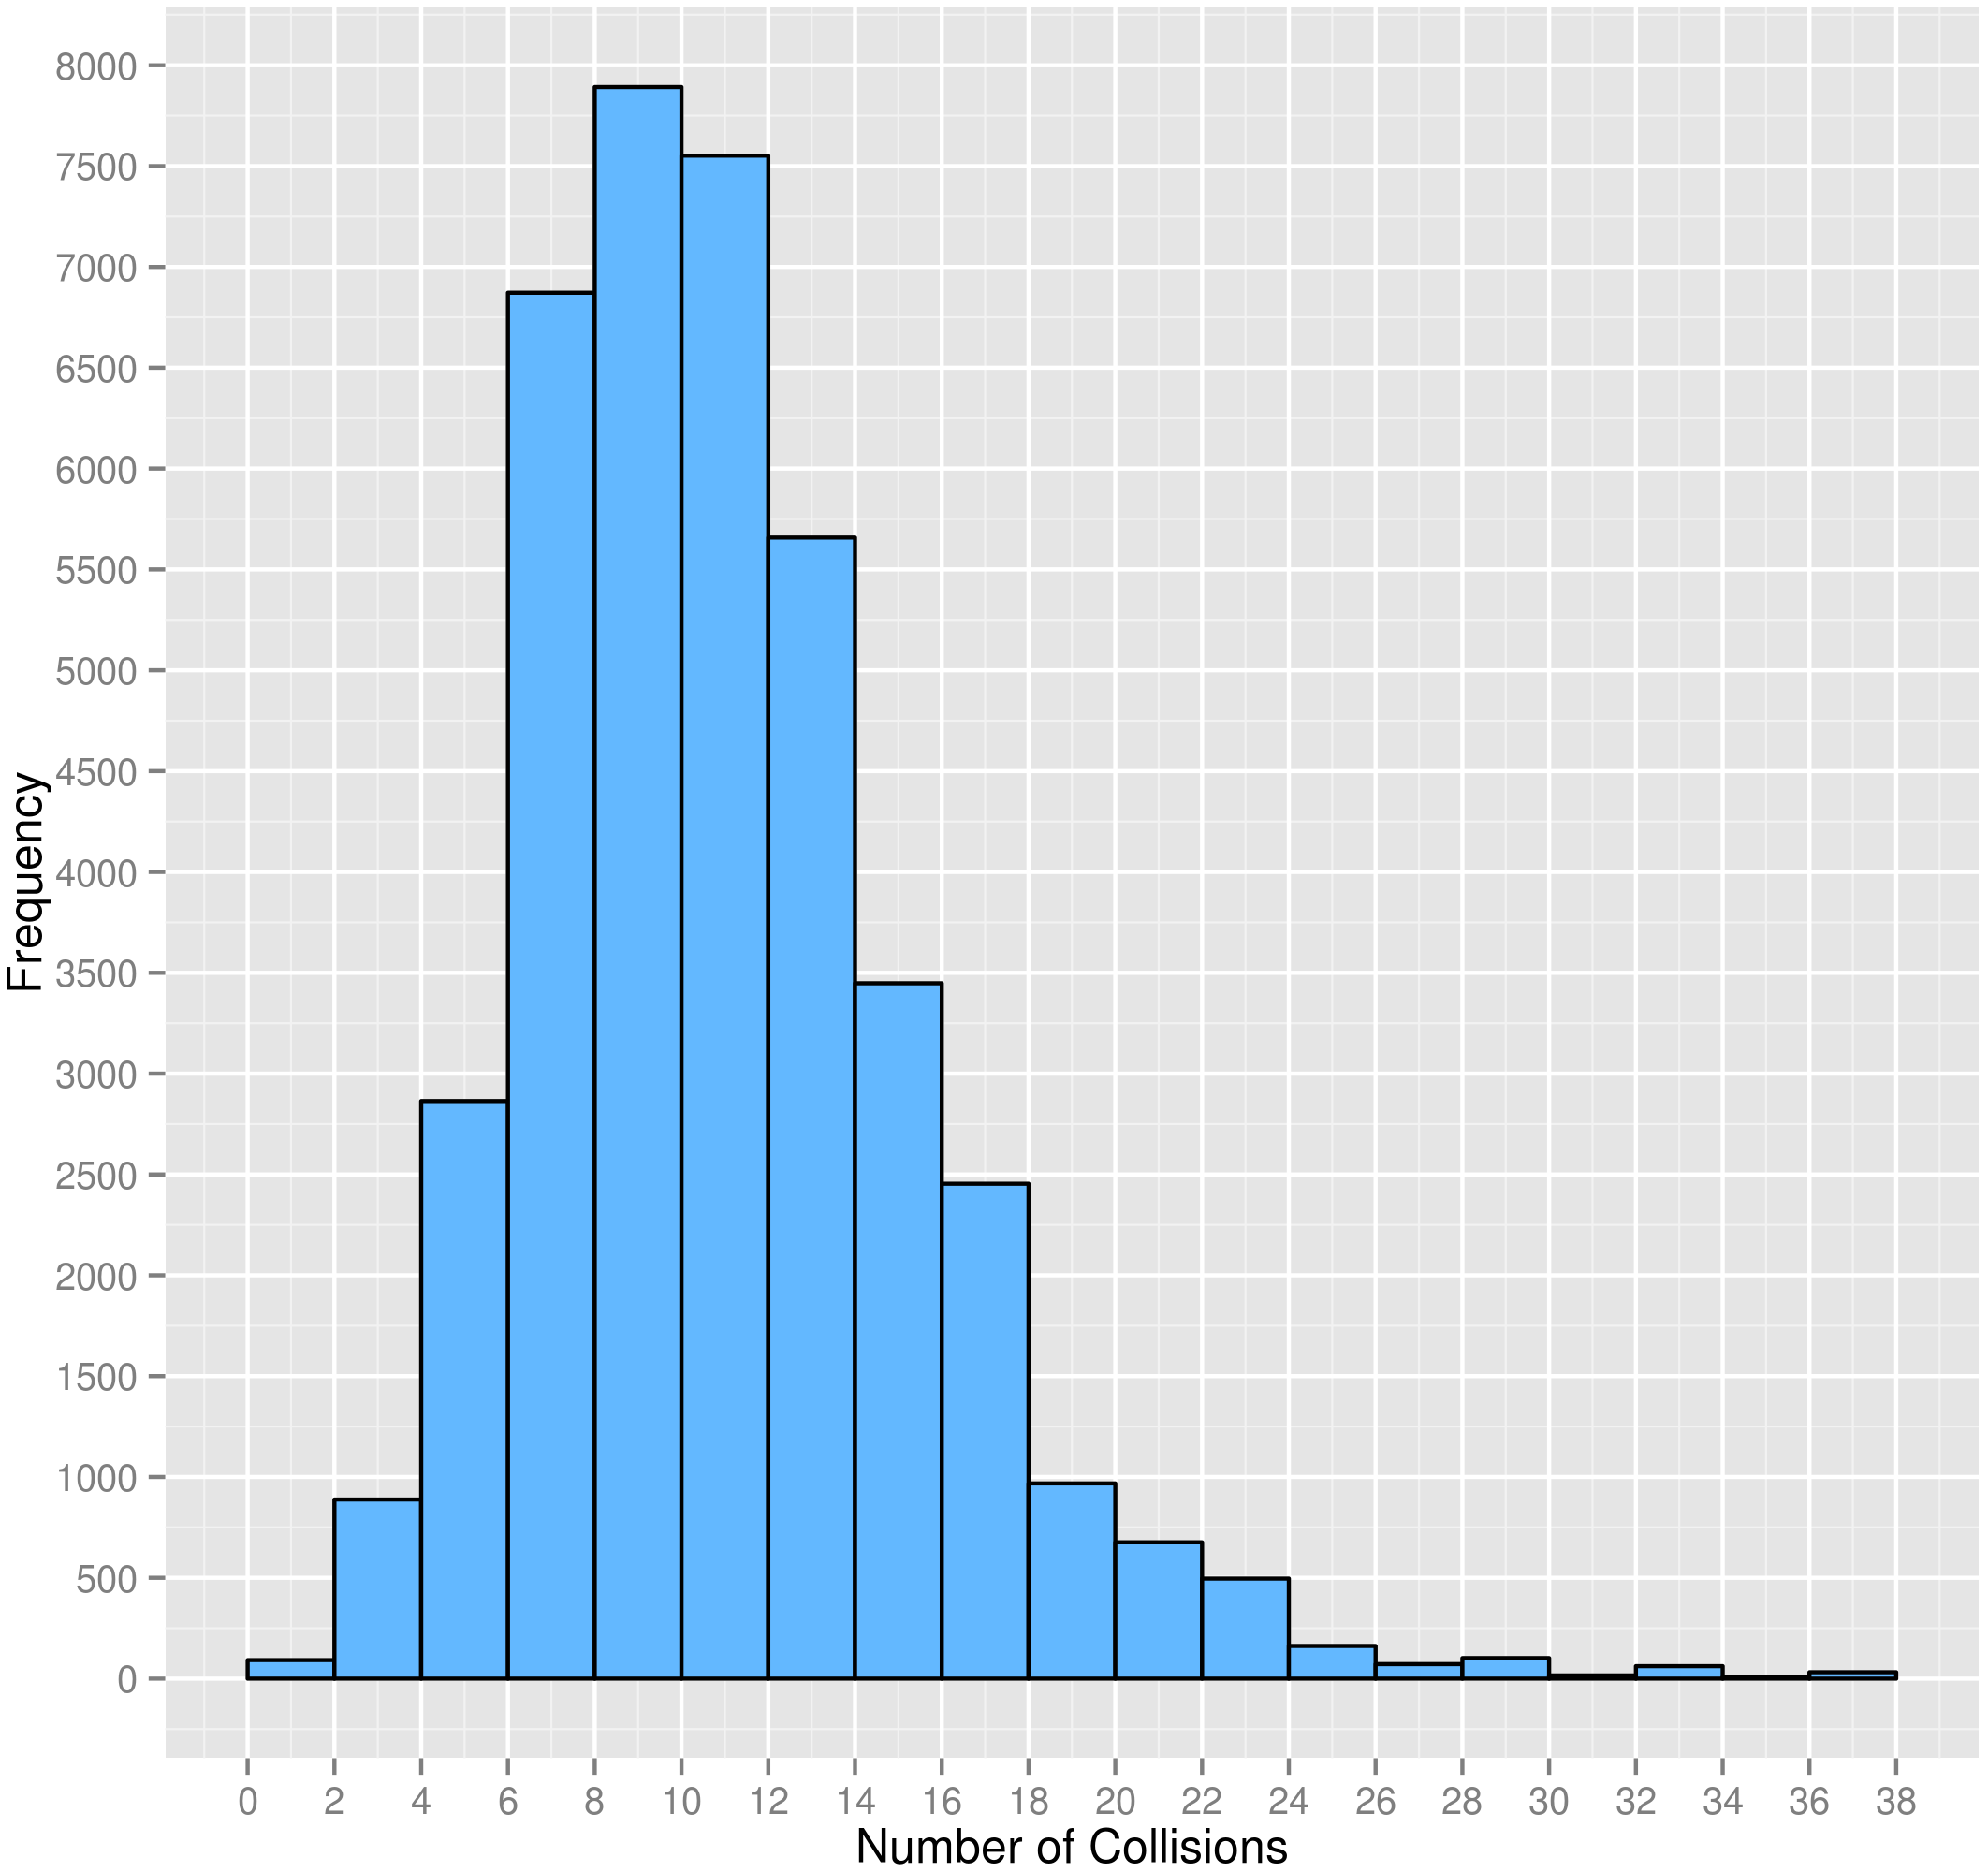
\includegraphics[width=0.45\textwidth]{figures/8_queens_histogram.png}}
\vspace{-12pt}
\caption{8-Queen Problem Collisions Histogram, Showing Distribution Based on Fitness Values}
\label{fig:histogram}
\end{figure}

8-Queen is the classical version of N-Queen. The histogram found in Figure \ref{fig:histogram} shows the full deterministic (brute force) traversal of the 8-Queen problem landscape, which is characteristic of the N-Queen problems. It details the myriad possibilities for the number of board states which can occur even in a relatively small problem size. Not pictured in this figure are the 4 instances of 44 simultaneous collisions, and 2 instances of 56 collisions. These occur when 7 or all 8 queens are all placed on the diagonals, respectively. Figure \ref{fig:histogram} clearly shows that the problem is highly multi-modal even for small problem sizes ($N = 8$). In this figure, 40228 local optima and 92 global optima are displayed, showing their distribution based on their fitness values.

While finding the most solutions given a fixed number of function calls/generations was the main objective of our proposed approach, fundamentally there are two variant objectives in tackling N-Queen problems. Finding the first solution as fast as possible is an alternative goal. The latter problem can be solved in polynomial time through conventional means \cite{cit:22,cit:23}, but finding as many solutions as possible is a challenging target which makes deterministic algorithms impractical.

\section{Related Work}
Deterministic attempts to solve N-Queen problems have been successful only for values of $N$ up to 26 \cite{cit:20}, and attempts to find single solutions quickly have been made for versions of the problem up to {$N = 500,000$} \cite{cit:21}. There are no known integer sequences or proofs which can represent the number of distinct solutions for $N > 26$, nor is there a deterministic means which can find them all within reasonable time frames. Traditional GAs have been used to find multitudinous solutions within fixed time frames \cite{cit:9,cit:10}. The same approach is utilized in our experiments.

Since tuning control parameters has a profound effect on the performance of GAs, one might conclude that there is an optimal static mutation probability \cite{cit:4} for solving N-Queen problems using the traditional approach. Hesser and M\"{a}nner \cite{cit:14} attempted to find such a value for GA in general problems but failed, because they are problem oriented values. Finding the pragmatic best case scenario for fixed mutation probabilities ($M_{c}$) within traditional GA proved to be useful for comparison in our experiments, which can be seen in our results.

Other alternative approaches to enhancing GA for combinatorial optimization sought to increase population diversity in order to overcome wasteful convergence to local optima, which is problematic in N-Queen since it has a huge number of local and global optima. This behavior prevents the search from finding more solutions. Combining standard GA with randomly generated individuals into the population is well studied \cite{cit:12}, but fails to adapt to suit the problem size. Still, exploring the nature of genetic diversity provides valuable insight into the motivation for increasing diversity among candidate solutions during the search process dynamically.

Adaptive GAs have historically manipulated control parameters by changing the mutation probability over time \cite{cit:12} such that it is high during exploration or low during exploitation. Other approaches used the overall mean population fitness to adjust genetic operators independent from time \cite{cit:11,cit:15,cit:7}. Alternative adaptive approaches have changed mutation probabilities between two values based on fitness values \cite{cit:15}, while others attempted to individually specify genetic operator probabilities for each phenotype, encoded with meta-operators that govern their evaluations \cite{cit:5}. Many previous adaptive approaches sought to yield more fruitful explorations of the problem landscape by tuning GA control parameters, but most approaches have been limited by being na\"{i}ve to either the problem size or the state of exploration and diversity. However, these historical adaptive methodologies yield many advantages over traditional GA in that they preclude the need for \textit{a priori} knowledge about optimal control parameters, mitigating the need to `tune them up' with protracted test runs prior to long-term evaluation, which saves time.

\section{Proposed Approach}
Our main motivation for this new self-adaptive approach was to leverage the observed tendency in nature for mutations to occur as a result of inbreeding with genetically similar specimens \cite{cit:17,cit:18}. Nature adjusts the mutation rate based on the diversity of the population. Our desire was to replicate this behavior in GA. We noted that mutations that resulted from inbreeding increased genetic diversity in biological organisms, affecting their fitness in nature sometimes for better or for worse. Therefore, it stood to reason that a similar phenomenon might occur in GA. Exploring this idea yielded surprisingly positive results.

\subsection{Chromosome Structure}
\label{section:chromosomestruct}
We used a GA with an integer-encoded chromosome to represent the N-Queen positions on the chessboard for all of our tests independent of their approach. Our chromosome structure includes protective embedded constraints which reduce the size of the search space drastically. These constraints are imposed through our data structure, which consists of a 1-dimensional array (of size $N$ with zero-based numbering) that stores the column position of the queens at each array index. The index is used to represent the row position of each queen, preventing more than one queen from appearing in the same row. Values stored inside the array must be between 0 and $N - 1$, preventing a queen from being placed outside the chessboard. However, we do not restrict the values within the array from being repeated, which can occur as a result of the crossover or mutation operators. When repetition occurs within the array, a collision will occur on the respective column. Our implementation uses traditional GA operators - selection, crossover, and mutation. Ordinary roulette wheel selection \cite{cit:19} is used in conjunction with single-value uniform mutation and single-point crossover/recombination \cite{cit:16}. 

% TABLE - EXPERIMENTAL VARIABLES
% TODO HAVE SHAHRYAR LOOK OVER THE VARIABLES/NAMING USED
\begin{table}
\centering
\caption{Experimental Control Parameters}
\begin{tabular}{|l|l|} \hline
Variable&                                     Value \\ \hline
Similarity Threshold ($S_{t}$)&               $15\%$ \\ \hline
Adaptive Mutation Bounds ($M_{a}$)&           $[1, 99]$ \\ \hline   
Adaptive Mutation Increment ($M_{a\Delta}$)&  $1$ \\ \hline
Crossover Probability ($P_{crossover}$)&      $70\%$ \\ \hline
Cloning Probability ($P_{cloning}$)&          $30\%$ \\ \hline
Population Size ($P$)&                        $64$ \\ \hline      
\end{tabular}
\label{table:geneticoperators}
\end{table}

\subsection{Self-Adaptive Mutation}
Chromosome similarity is used as a main feature in our adaptation approach. The probability for the mutation operator is dynamically adjusted, while recombination ($P_{crossover}$) remains at a single static value as in traditional GA. Our experimental settings for the genetic operators are given in Table \ref{table:geneticoperators}.

In order to apply our self-adaptive mutation approach, a two step process is required. First, each generation's chromosomes' similarity must be evaluated. The similarity algorithm is detailed in Algorithm \ref{alg:similarity}. Next, the mutation probability is adjusted accordingly in order to adapt. This allows the population to be diversified when it is required to improve the search.

When the chromosome similarity is less than the specified threshold ($S_{t}$), the population is too dissimilar (high diversity). This means the mutation probability must decrease, because the population is not inbred. For the next generation, the mutation probability is subtracted by $M_{a\Delta}$ indicated in Table \ref{table:geneticoperators}. After application of genetic operations and selection on the population, the next generation is populated and their chromosome similarity is calculated. If the chromosome similarity has increased, and if it is ever above the specified threshold, the population is inbred. $M_{a}$ must increase by the fixed delta in the next generation to adapt.

Variations in chromosome similarity may result independently of the applied uniform mutation operator. Since the recombination probability ($P_{crossover}$) is 70\%, the recombinant permutations are likely to be approximately 30\% similar (due to cloning) unless uniform mutation has occurred on the cloned genes. Our experimental observations indicate that when using adaptive mutation the chromosome similarity will approach an equilibrium percentage approximately equal to the specified similarity threshold ($S_{t}$) as generations evolve.

\subsection{Chromosome Similarity Algorithm}
Chromosome similarity is calculated using a deterministic algorithm, presented in Algorithm \ref{alg:similarity}. First, the chromosomes' genes are decoded and re-encoded into integer values and concatenated into one large integer. Next, the resultant array of integer representations is sorted. Our implementation uses the quick-sort algorithm provided by Java for minimal computational overhead. This gives the similarity algorithm its characteristic asymptotic behavior, as the complexity of the sorting function itself is of higher complexity than the rest of the main similarity calculation algorithm. Quick-sort runs in $O(n \log n)$ complexity, although it should be noted that in the theoretical worst case, quick-sort works in $O(n^2)$ which is highly unlikely. The main algorithm runs in $O(n)$ linear complexity independent of the sorting. Similar chromosomes have the same genes. A population with 100\% similarity is completely identical.

\begin{algorithm}
  \SetKwProg{Fn}{Function}{}{end}\SetKwFunction{Similarity}{Similarity}%
  \SetKwData{Similar}{similar}\SetKwData{Value}{value}\SetKwData{Matched}{matched}\SetKwData{Length}{length}\SetKwArray{Sorted}{sorted}
  \SetKwFunction{Sort}{Sort}
  \SetKwInOut{Input}{input}\SetKwInOut{Output}{output}
  \SetAlgoLined
  \DontPrintSemicolon
  
  \Fn{\Similarity{$chromosomes$}}{
  
  \Input{An array of $chromosomes$}
  \Output{Fraction of chromosomes that are similar}
  \BlankLine
  
  \Similar $\leftarrow$ 0\;
  \Matched $\leftarrow$ false\;
  \Length $\leftarrow$ length of $chromosomes$\;
  \BlankLine
  
  \tcp{Sort using an arbitrary sorting algorithm}
  \Sorted $\leftarrow$ \Sort{$chromosomes$}\;
  \BlankLine
  
  \For{$i \leftarrow 0$ \KwTo $\Length -1$}
  {
    \uIf{\Sorted{$i$} == \Sorted{$i + 1$}}
    {
      \Similar $\leftarrow$ \Similar + 1\;
      \Matched $\leftarrow$ true\;
    }
    \ElseIf{\Matched}
    {
      \Similar $\leftarrow$ \Similar + 1\;
      \Matched $\leftarrow$ false\;
    }
    \BlankLine
    
    \tcp{Case where the last item is a match}
    \If{\Matched and $\left(i + 1 == \Length - 1 \right)$}
    {
      \Similar $\leftarrow$ \Similar + 1\;
    }
  }
  \BlankLine
  \KwRet{\Similar / \Length}
  }
\caption{Chromosome similarity evaluation function}
\label{alg:similarity}
\end{algorithm}

\subsection{Fitness Function}
Candidate solution fitness is evaluated by determining the number of collisions ($C$) between queens on the chessboard. This means that in a board state where one queen can attack another, two collisions result. When three queens can attack another, 6 collisions result. The algorithm for determining the fitness of a given board state is given in Algorithm \ref{alg:fitness}, showing the mechanisms used to find collisions across diagonals on the board. The overall board state fitness is calculated as $fitness = \frac{1}{C}$, where $fitness = 1$ if $C = 0$. Maximum fitness is achieved when $C = 0$ as there are no collisions, resulting in a distinct board solution. For example, in the classical 8-Queen problem, the ideal fitness is 1, and the worst case fitness is $1/56$.
 
\begin{algorithm}[t!]
  \SetKwProg{Fn}{Function}{}{end}\SetKwFunction{Fitness}{Fitness}%
  \SetKwData{Collisions}{collisions}\SetKwData{Length}{length}\SetKwArray{Chromosome}{$chromosome$}\SetKwData{Yi}{$y_i$}\SetKwData{Yj}{$y_j$}
  \SetKwFunction{Abs}{abs}
  \SetKwInOut{Input}{input}\SetKwInOut{Output}{output}
  \SetAlgoLined
  \DontPrintSemicolon
  
  \Fn{\Fitness{$chromosome$}}
  {
    \Input{A single $chromosome$}
    \Output{A fitness value for the chromosome}
    \BlankLine
    
    \Collisions $\leftarrow$ 0\;
    \Length $\leftarrow$ length of the $chromosome$\;
    \BlankLine
    
    \For{$i \leftarrow 0$ \KwTo $\Length -1$}
    {
      \tcp{Check each gene against the current}
      $j \leftarrow \left( i + 1 \right) \mod{\Length}$\;
      \While{$j$ != $i$}
      {
        \Yi $\leftarrow \Chromosome{i}$\;
        \Yj $\leftarrow \Chromosome{j}$\;
        \BlankLine
        
        \tcp{Check for vertical collision}
        \If{\Yi == \Yj}
        {
          \Collisions $\leftarrow \Collisions + 1$\; 
        }
        \BlankLine
        
        \tcp{Check for diagonal collision}
        \If{\Abs{$\left(i - j \right)$ / $\left(\Yi - \Yj \right)$} == 1}
        {
          \Collisions $\leftarrow \Collisions + 1$\;
        }
        \BlankLine
        
        $j \leftarrow \left(j + 1 \right) \mod{\Length}$\;
      }
    }
    \BlankLine

    \eIf{\Collisions == 0}
    {
      \KwRet{1}\;
    }
    {
      \KwRet{1 / \Collisions}\;
    }
  }
\caption{Fitness function}
\label{alg:fitness}
\end{algorithm}

\subsection{Identifying Distinct Solutions}
In each generation there is always a strong possibility that some of the chromosomes in the current population are valid solutions - any of the current generation's chromosomes with a fitness of 1 is some sort of solution. Whether it is distinct or not is unknown at first. When a solution is found, it must be compared to the list of previously found solutions to determine whether it is distinct. Symmetry operations are applied to each solution found to generate more distinct solutions based on the symmetrical nature of the chessboard. This may further increase the likelihood that the new population's solutions have already been found previously. Therefore, indistinct solutions are discarded without having symmetry operations applied as their reconfiguration would already be identical to symmetric configurations of previously found distinct solutions. After saving newly found solutions, the new generation replaces the previous generation and the GA continues.

Symmetry operations consist of three $90^{\circ}$ rotations, a horizontal reflection, and then 3 further $90^{\circ}$ rotations of the reflected board. Each symmetrical board configuration is a candidate solution that is checked against the existing distinct solutions. It is discarded if it has already been found previously, because it is indistinct. Each distinct solution can potentially yield up to 7 additional distinct solutions depending on the placement of queens.

\section{Experiments}
We measured the performance of our self-adaptive approach using an empirical study. Our methodology was to solve N-Queen problems for various values of N with a limited budget of function calls (generations), repeated a multitude of times to ensure accuracy and collect aggregate statistics. Table \ref{table:trials} shows the number of function calls permitted and the number of trials run for each value of N. Special budgets and trial multiplicities were set for $N = 32$ in order to accommodate the exceptionally large problem size.

Our control used traditional GA with fixed mutation probabilities ($M_{c}$) of $M_{c}$ = 1\%, 5\%, 10\% to 100\% (with a step size of 5\%) to solve each N-Queen problem. These trials were run with the same multiplicity and budget as our self-adaptive approach. The goal of the control trials was to approximately determine the optimal $M_{c}$ for finding the most solutions for each problem in the given time budget, and finding the first solution fastest. Our aim was to test our new approach against a reasonable approximation of the best possible performance that the traditional GA approach can provide. Optimized control parameters for mutation would be determined and used as a benchmark, similar to Hesser and M\"{a}nner's study \cite{cit:14}.

% TABLE - EXPERIMENTAL TRIALS/TESTS
% TODO HAVE SHAHRYAR LOOK OVER THE VARIABLES/NAMING USED
\begin{table}
\centering
\caption{Experimental Trials}
\begin{tabular}{|l|l|l|} \hline
$N$&        Budget (Generations)&     Trials \\ \hline
8&          10,000,000&         30 \\ \hline
9&          10,000,000&         30 \\ \hline
10&         10,000,000&         30 \\ \hline
11&         10,000,000&         30 \\ \hline
12&         10,000,000&         30 \\ \hline
13&         10,000,000&         30 \\ \hline
14&         10,000,000&         30 \\ \hline
15&         10,000,000&         30 \\ \hline
16&         10,000,000&         30 \\ \hline
18&         10,000,000&         15 \\ \hline
20&         10,000,000&         15 \\ \hline
22&         10,000,000&         15 \\ \hline
24&         10,000,000&         15 \\ \hline
26&         10,000,000&         15 \\ \hline
32&         50,000,000&         10 \\ \hline
\end{tabular}
\label{table:trials}
\end{table}

Given the increasingly large problem sizes, the number of tests were reduced in order to allow experimentation to complete within reasonable time frames. Descriptive statistics were gathered every 1000 generations, with mean calculated using the grand mean.

\section{Results and Analysis}
The performance difference with respect to the number of found solutions can be seen in Table \ref{table:distinctsol}. The traditional GA approach performs marginally better in the range of small problems, which are most efficiently solved with deterministic methods. This range consists of values of $N \leq 14$. Our self-adaptive approach yields more solutions for values of $N$ where $N > 14$. As $N$ increases, the difference widens; the self-adaptive approach provides increasingly better results for this objective as the problem size increases.

We observed that there is a proportional inverse relationship between $N$ and the best experimentally determined $M_{c}$. As $N$ increases, the best $M_{c}$ which yielded the most solutions decreases. The point this raises is that there is an unfair advantage for the traditional GA over the self-adaptive approach, since the optimal static $M_{c}$ changes as $N$ changes. But we know that the ideal $M_{c}$ for all problems are unknown. Generally, foreknowledge of the ideal $M_{c}$ is not available in order to exploit this advantage \cite{cit:14}, but in this case it was experimentally determined. Optimally tuned control parameters are critical and provide a major advantage. Still, the self-adaptive approach consistently outperformed traditional GA with optimized parameters for the large problem sizes, even as the parameters were adjusted to better suit the problem. Our conclusion is that the self-adaptive approach will continue to outperform the traditional GA method as $N$ grows, based on the increasing gap in performance observed. The main reason is that even the most optimal value of the mutation rate remains unchanged during the search process. This is why it cannot compete with our self-adaptive scheme.

\begin{figure}[htp]
\centerline{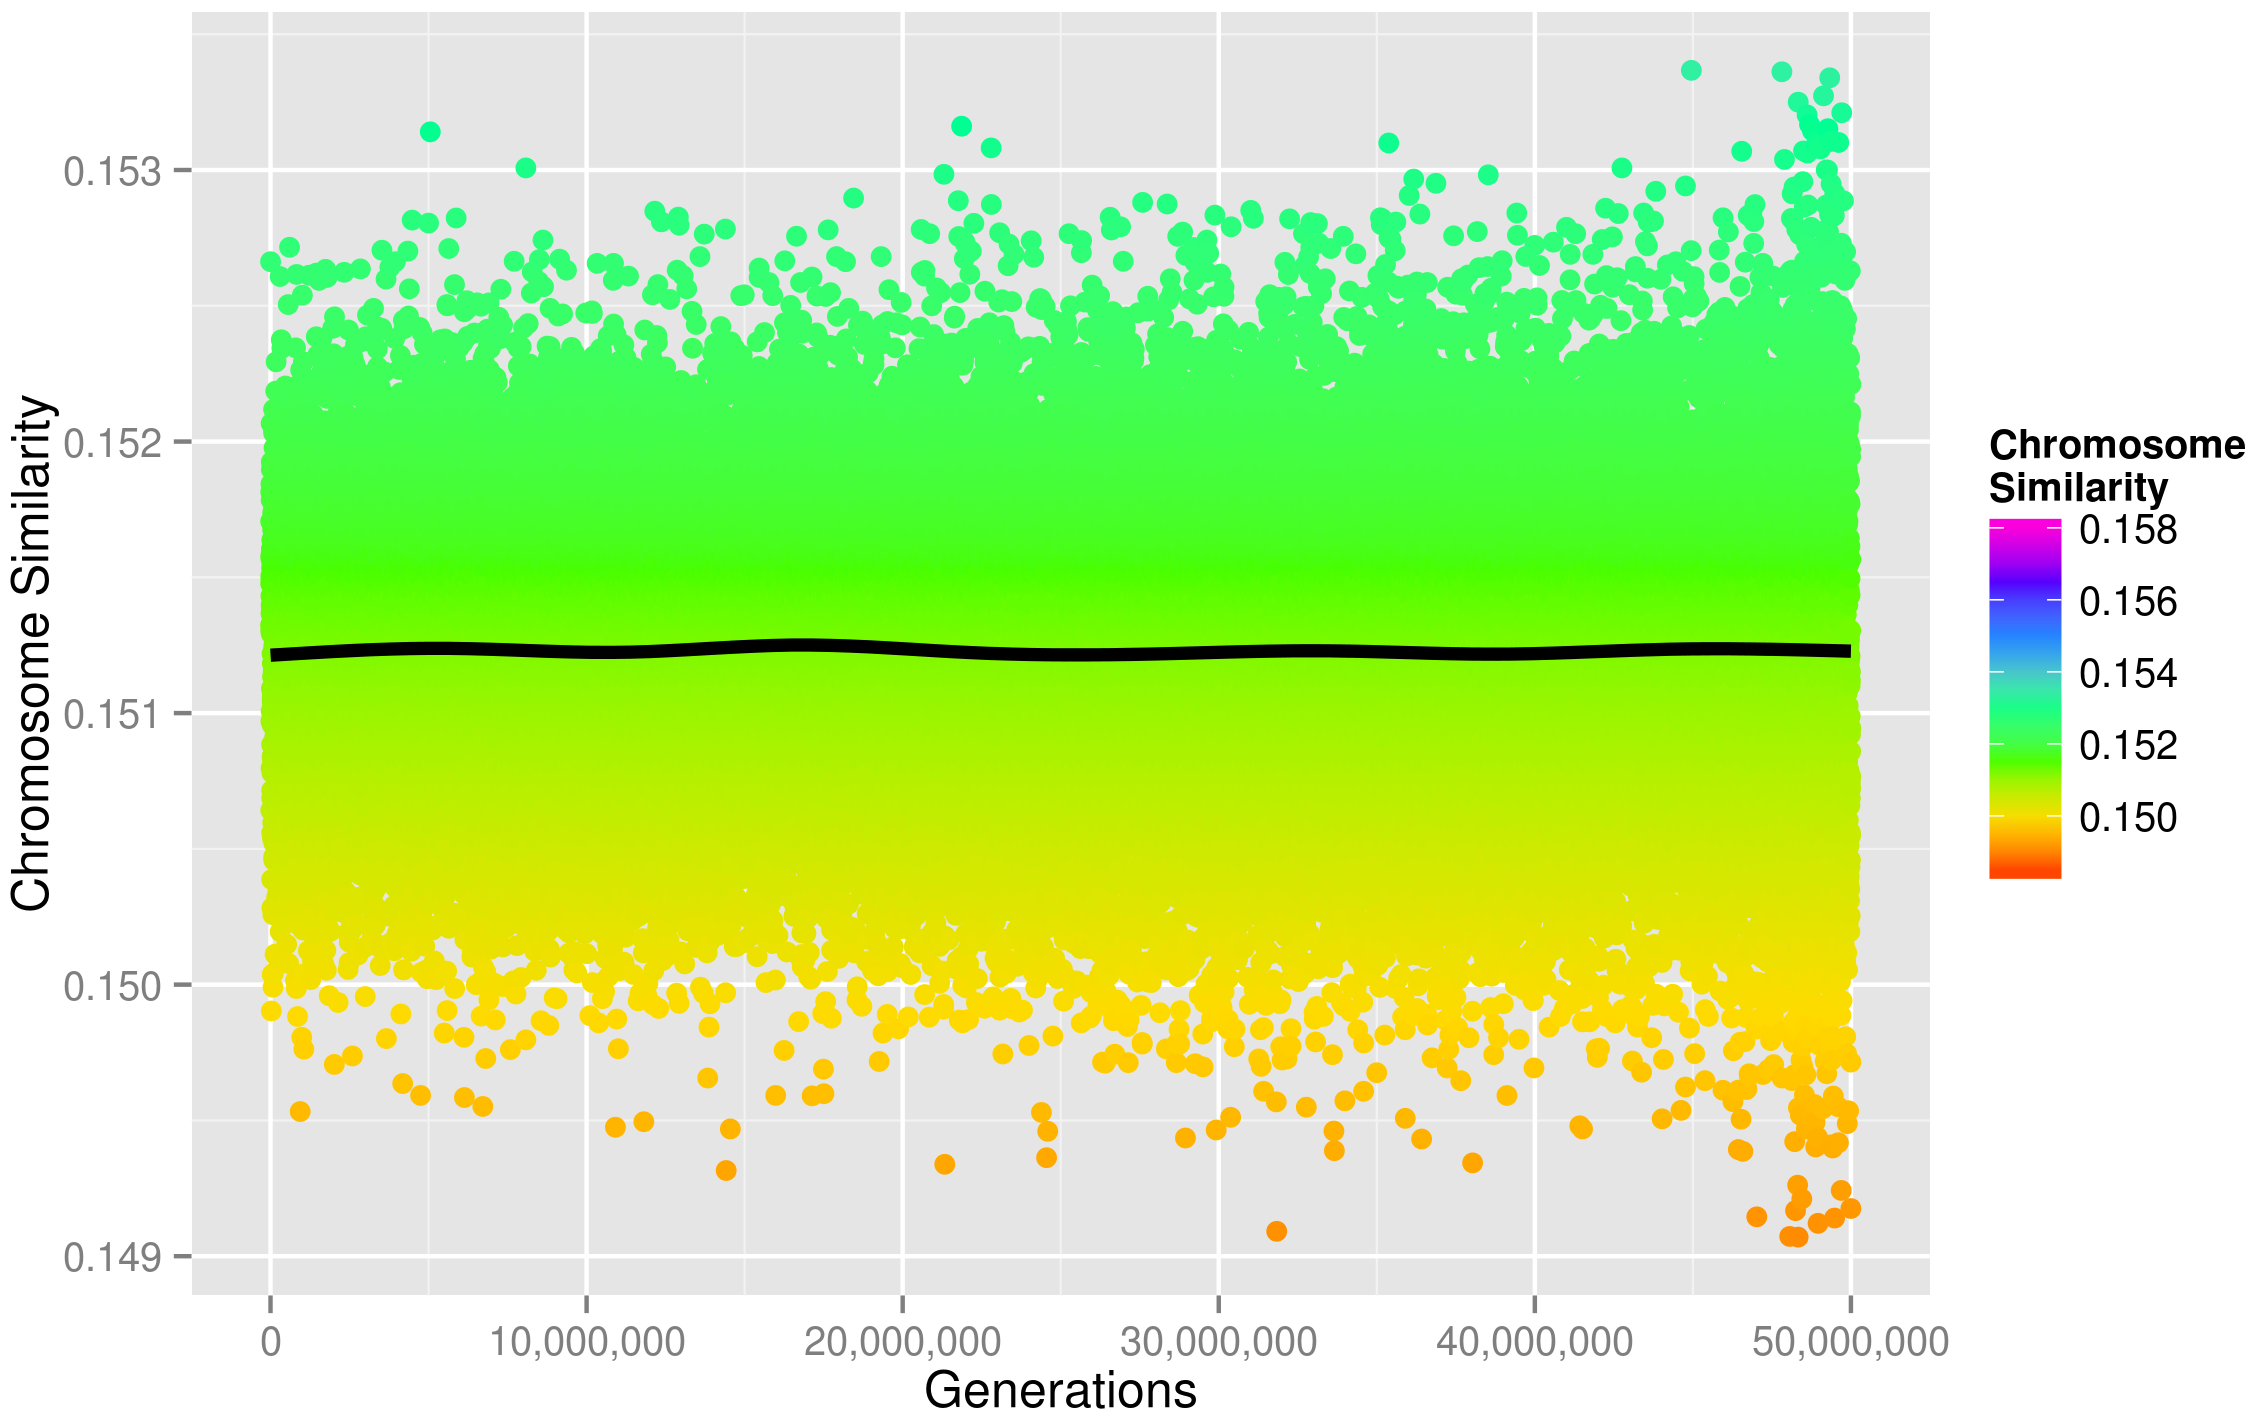
\includegraphics[width=0.48\textwidth]{figures/similarity_variable_32q_3.png}}
\vspace{-6pt}
\caption{Chromosome Similarity vs Generations for the 32-Queen Problem (Self-Adaptive)} 
\label{fig:sim32q}
\end{figure}

\begin{figure}[htp]
\centerline{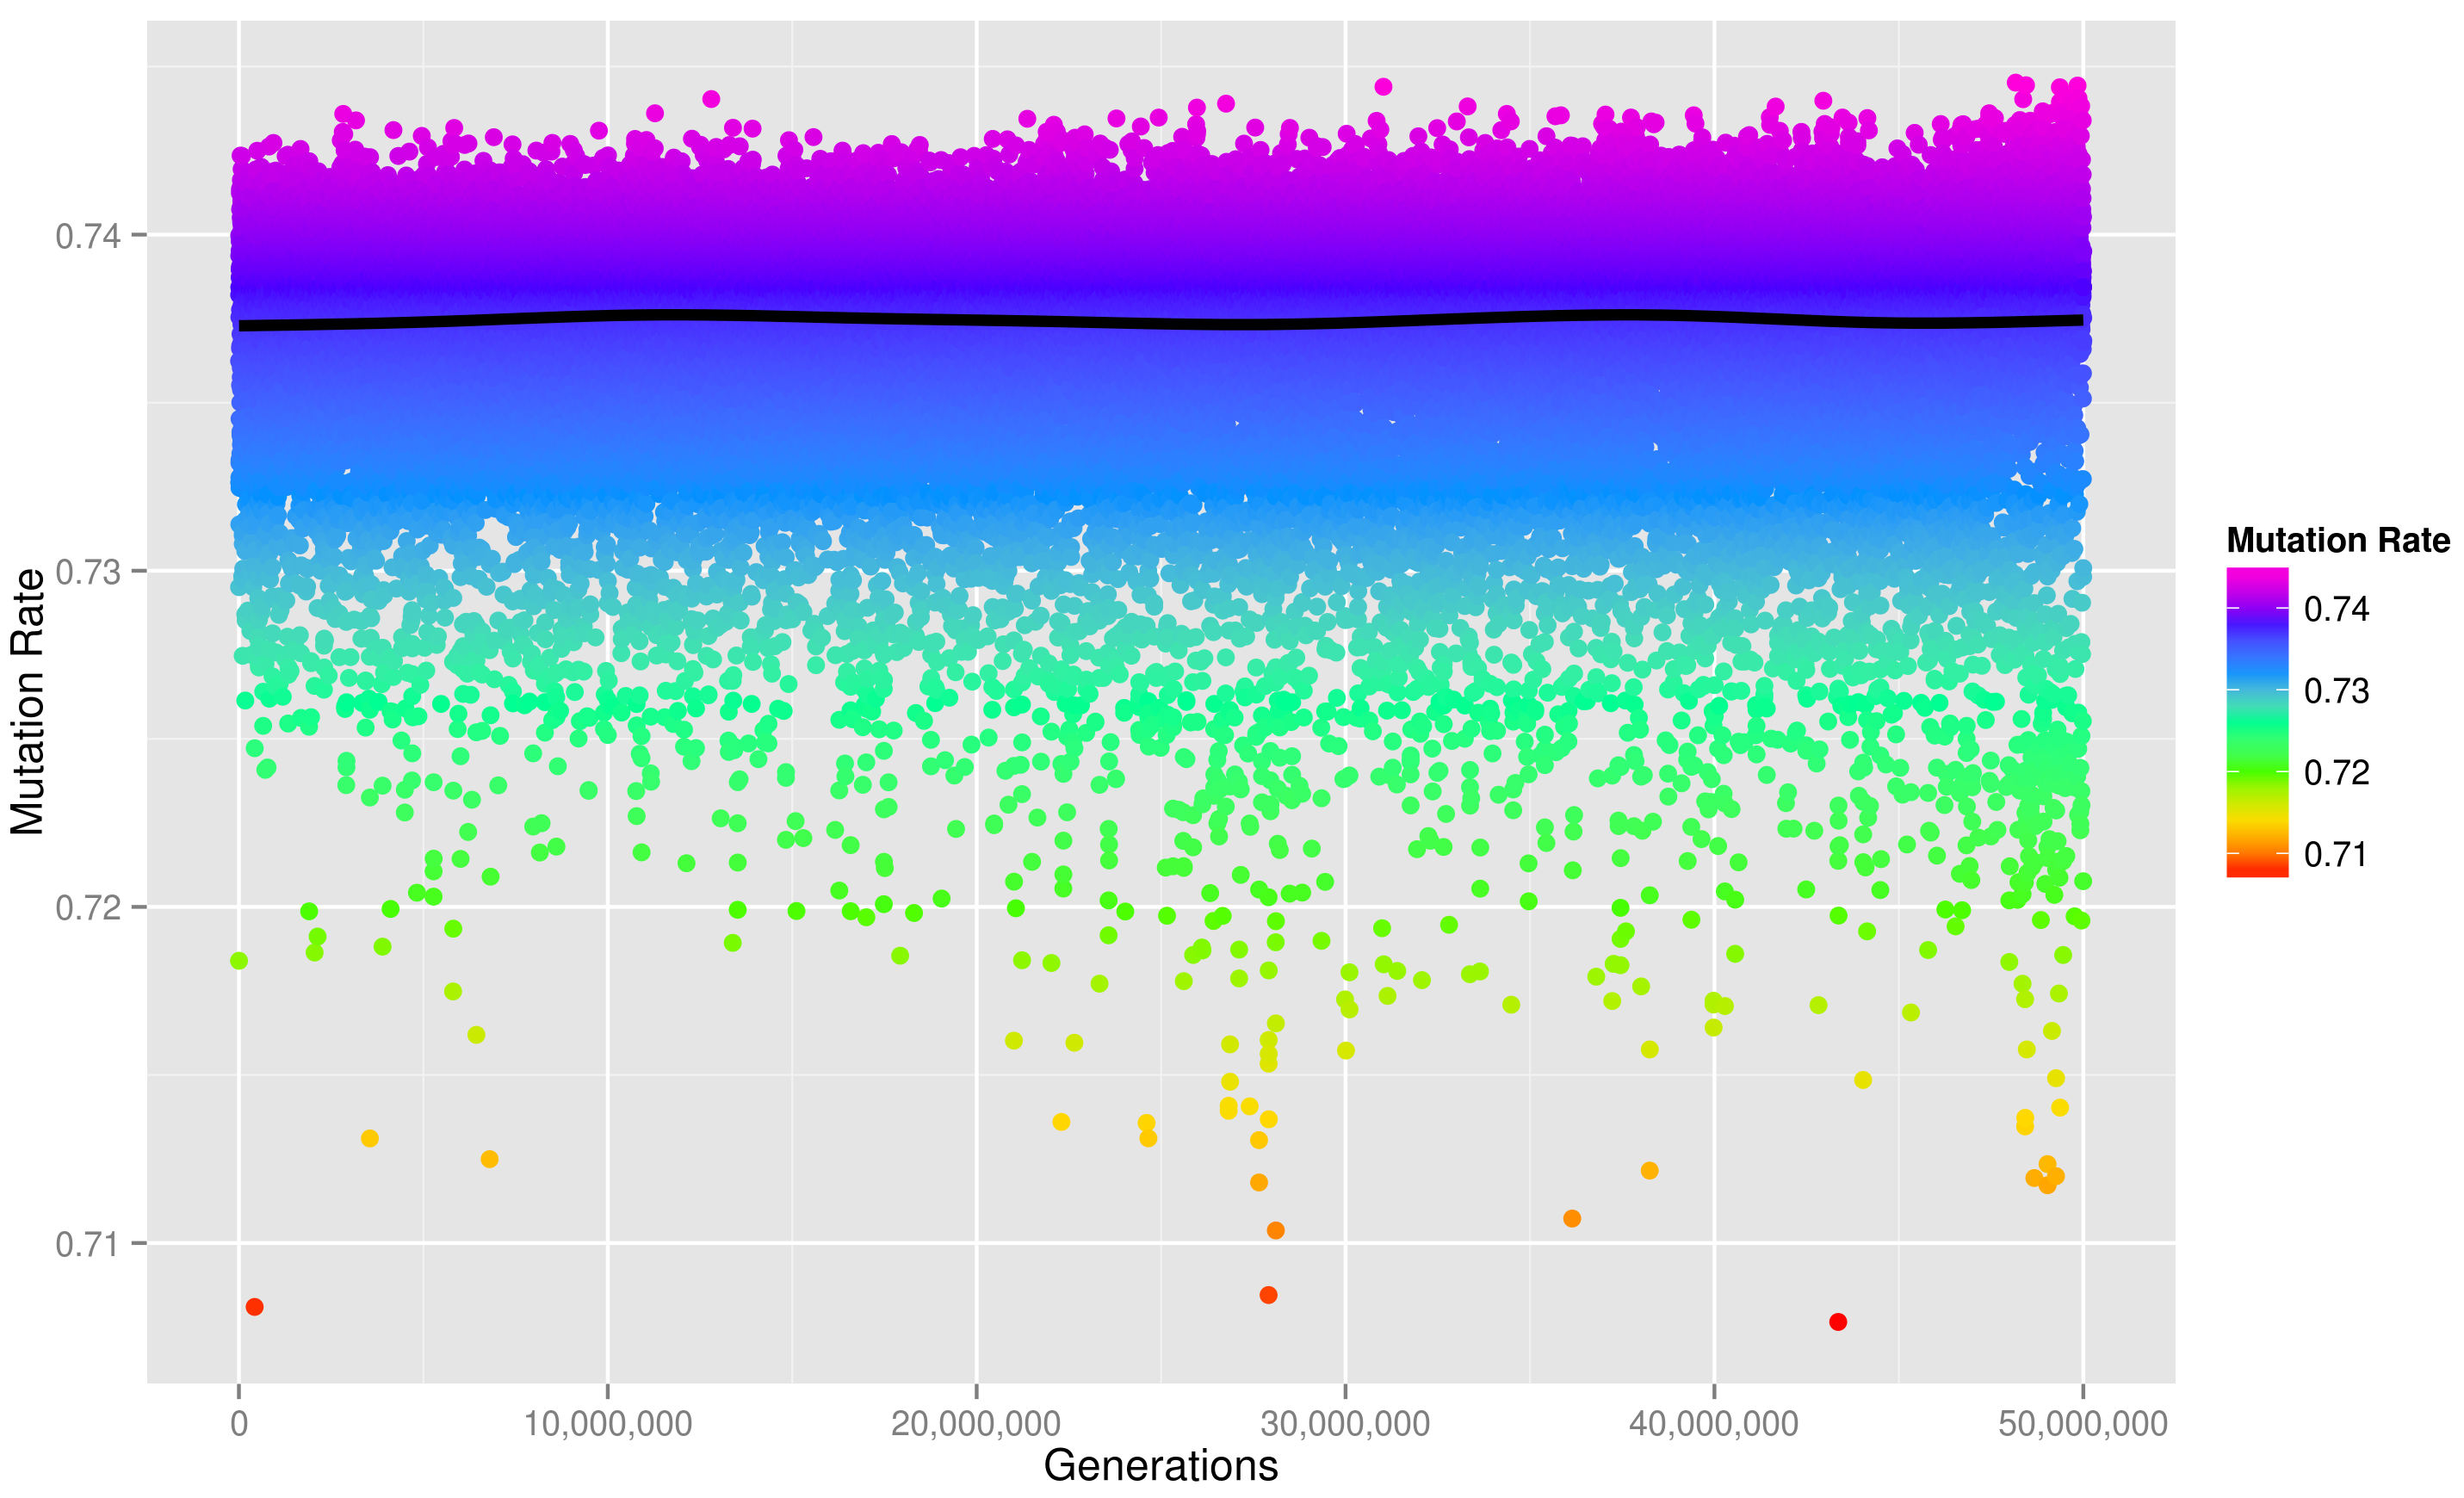
\includegraphics[width=0.48\textwidth]{figures/mutation_32q_1.png}}
\vspace{-6pt}
\caption{Mutation Probability vs Generations for the 32-Queen Problem (Self-Adaptive)} 
\label{fig:mutation32q}
\end{figure}

Our analysis of the algorithm shows that the self-adaptive approach adjusts the mutation probability throughout the duration of the solution search. In contrast to historical approaches, the adaptive approach does not adapt based on one characteristic of the problem, the stage of the search, position of the individuals on the landscape, or fitness values. Our results also show that adaptation occurs every generation, since stochastic factors routinely influence the similarity beyond or below the similarity threshold ($S_{t}$). This behavior can be seen in Figure \ref{fig:sim32q}, which shows that the chromosome similarity changes as a result of the mutation operator to approach the specified $S_{t}$. Figure \ref{fig:mutation32q} shows the corresponding changes in mutation probability over generations based on similarity. Comparatively, Figure \ref{fig:bestfixedn32q} shows the similarity over generations of the most optimal traditional mutation operator found for the 32-Queen problem, $M_{c} = 0.65$. At this mutation probability, traditional GA tends toward a similarity of $25\% \pm 1\%$, with lower and upper extrema at 1.8\% and 26.4\%. This lies in stark contrast to the self-adaptive approach which tended toward the specified $S_{t}$ at 15\%, using adaptive mutation probabilities that tended toward 73.7\% with lower and upper extrema at 70.8\% and 74.5\%.

\begin{figure}[htp]
\centerline{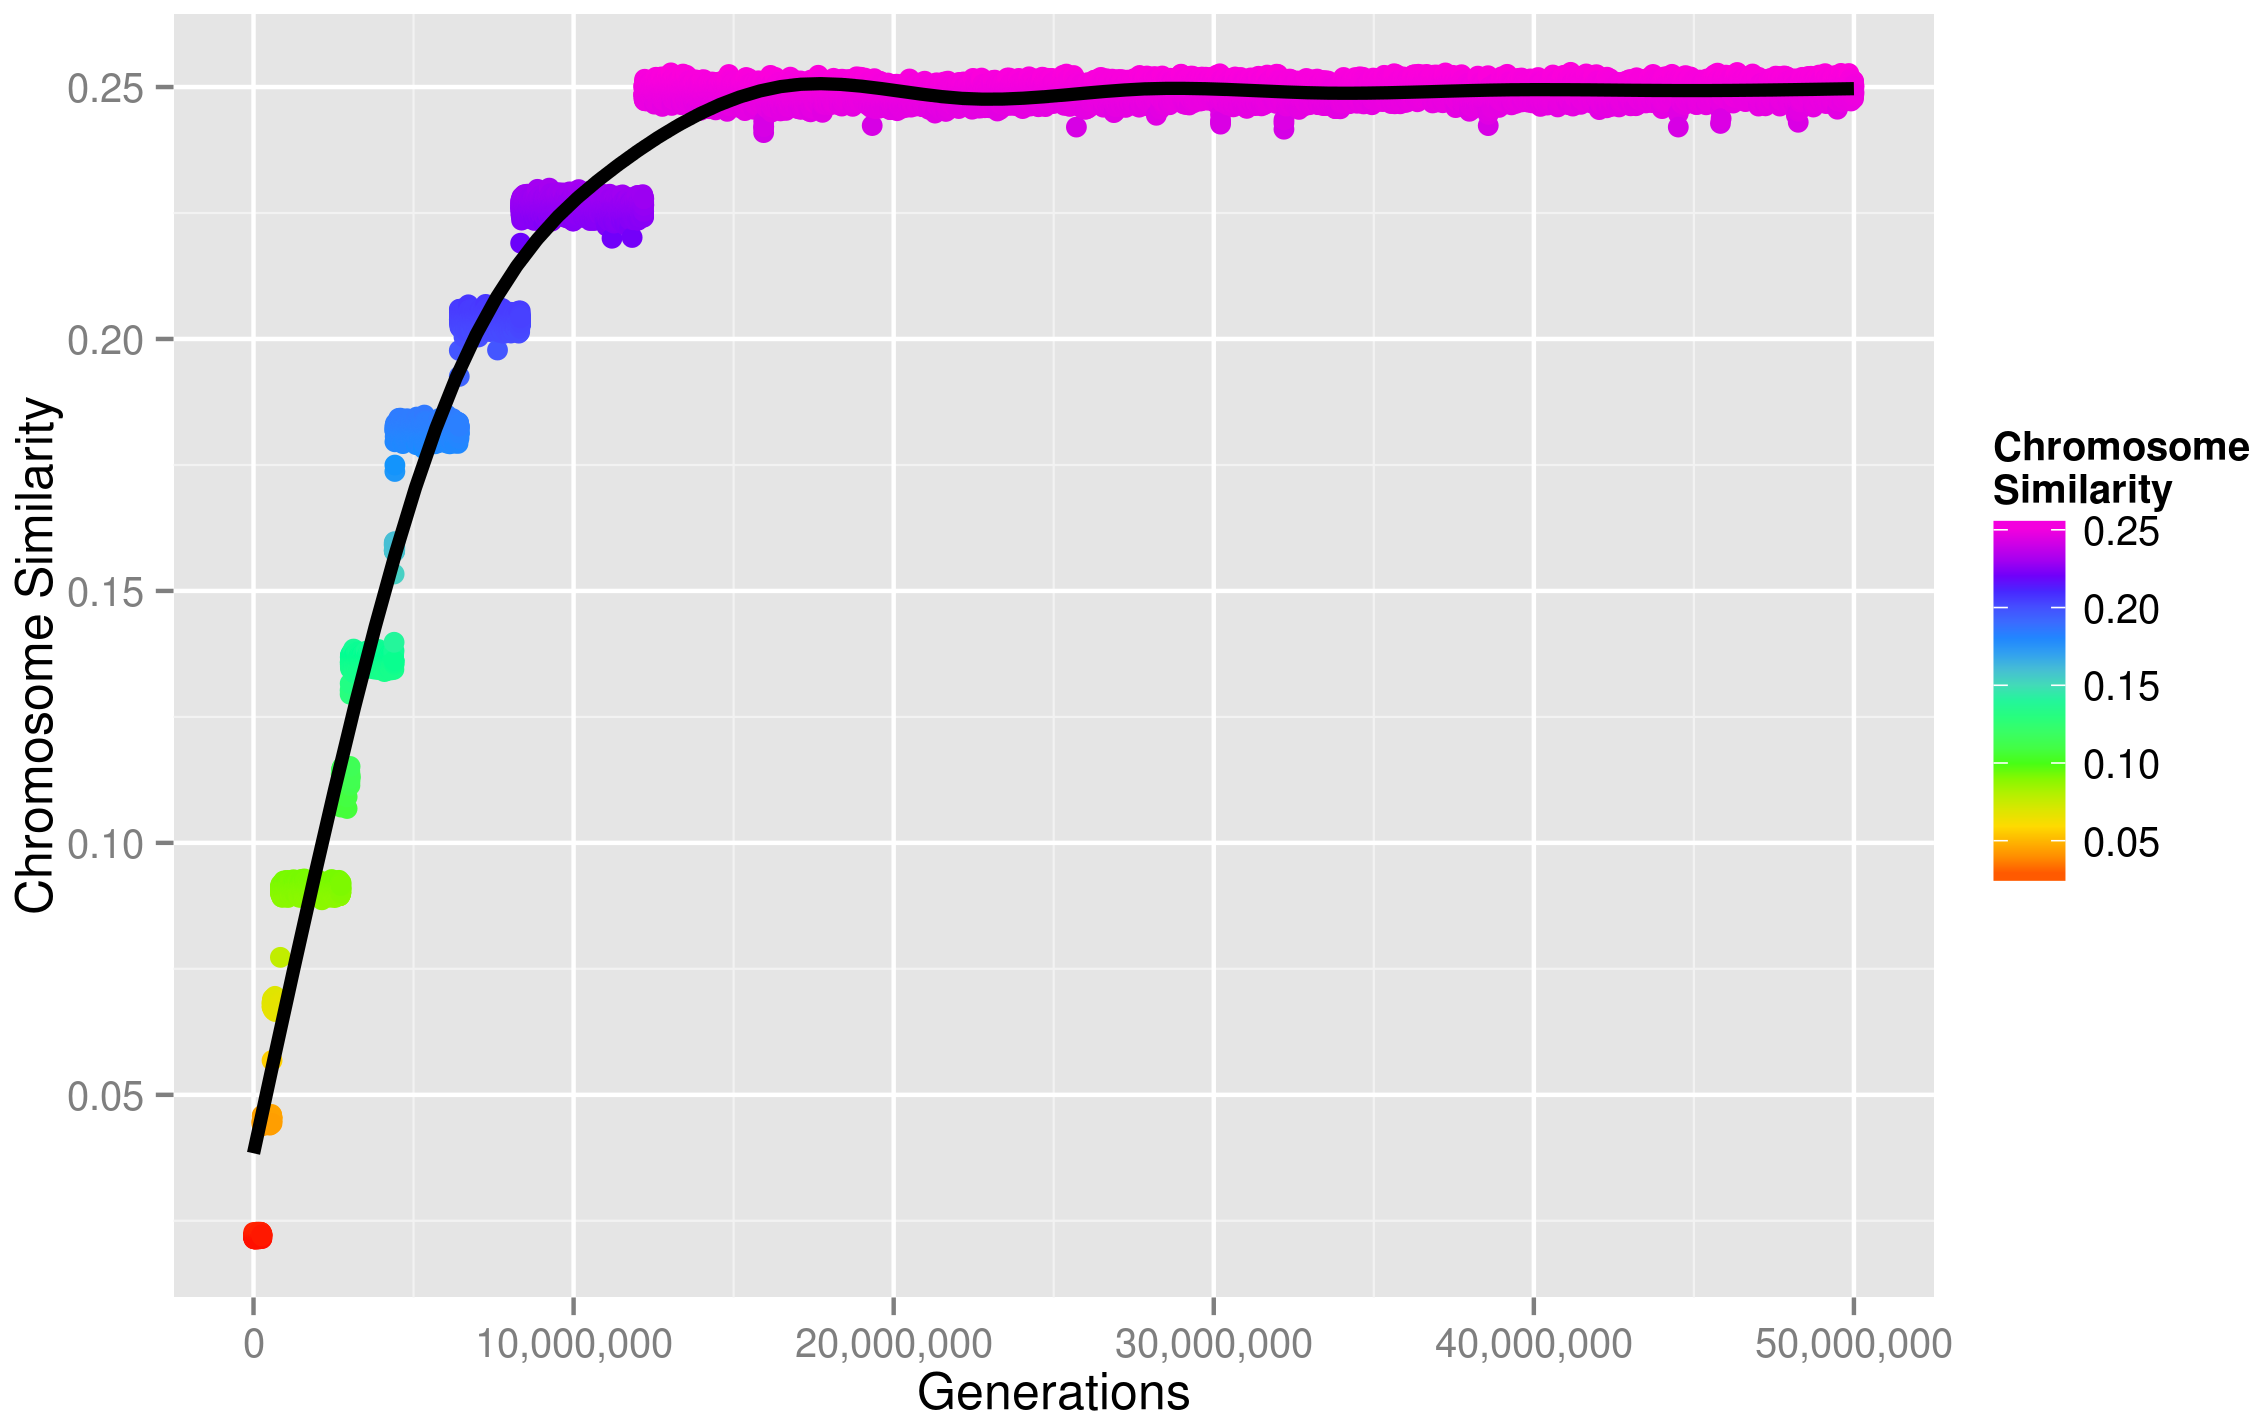
\includegraphics[width=0.48\textwidth]{figures/similarity_065_32q_3.png}}
\vspace{-6pt}
\caption{Chromosome Similarity vs Generations for the 32-Queen Problem (Traditional GA, $M_{c} = 0.65$)} 
\label{fig:bestfixedn32q}
\end{figure}

The self-adaptive approach increases diversity and generates more diverse candidate solutions for efficient traversal of the areas of the problem landscape that contain undiscovered solutions. The diversity is increased because the search is prevented from regenerating identical chromosomes, flooding the population with clones. Controlling similarity allows the self-adaptive approach to strike a balance between convergence, exploration, and exploitation. Therefore, there is a reverse relationship between diversity and chromosome similarity which enables the diversity of the population to be controlled by the specified threshold ($S_{t}$). In traditional GA, when the chromosome similarity is too high, diversity is low and few solutions are found. This is evident by the poor performance yielded by traditional GA in our benchmarks where $M_{c}$ is very small. There is no mechanism other than the constant background mutation that increases diversity among the population, since recombination of identical chromosomes results in a clone regardless. Conversely, when mutation is too frequent (such as in high values of $M_{c}$ like 100\%), similarity becomes low and the diversity of the population becomes too high to allow optima to be converged upon. The search algorithm turns into a random walk approach. When solutions are converged upon in the self-adaptive approach, diversity increases as the mutation rate adapts in order to expand the search to other unexplored regions of the landscape. This behavior is the desirable characteristic of the self-adaptive approach that makes it ideal for highly multi-modal problems with many optima like N-Queen problems. Controlled similarity prevents the GA from being stuck in a plateau of similar local optima, while also preventing the search from being wildly dissimilar and random, failing to converge on global optima.

\begin{table}
\centering
\caption{Most N-Queens Distinct Solutions}
\begin{tabular}{|l|l|l|l|l|} \hline
&               &  \multicolumn{2}{c|}{Distinct Solutions Found}& \\ \cline{3-4}
$N$&  Best $M_{c}$&  Best $M_{c}$&    Self-Adaptive ($M_{a}$)&    Difference\\ \hline
8&  0.95&          92&              92&                         $\pm$ 0\% \\ \hline                        
9&  0.95&          352&             352&                        $\pm$ 0\% \\ \hline
10& 0.9&           724&             724&                        $\pm$ 0\% \\ \hline
11& 0.85&          2,680&           2,680&                      $\pm$ 0\% \\ \hline
12& 0.85&          13,690&          11,986&                     $-$12.45\% \\ \hline
13& 0.8&           32,128&          26,308&                     $-$18.12\% \\ \hline
14& 0.8&           41,520&          29,520&                     $-$28.90\% \\ \hline
15& 0.8&           30,356&          30,324&                     $-$0.11\% \\ \hline
16& 0.8&           15,016&          30,132&                     $+$100.67\% \\ \hline
18& 0.75&          16,392&          27,120&                     $+$65.45\% \\ \hline
20& 0.75&          7,872&           25,608&                     $+$225.30\% \\ \hline
22& 0.7&           6,008&           25,376&                     $+$322.37\% \\ \hline
24& 0.7&           6,440&           24,560&                     $+$281.37\% \\ \hline
26& 0.7&           6,280&           23,008&                     $+$266.37\% \\ \hline
32& 0.65&          15,216&          104,080&                    $+$584.02\% \\ \hline
\end{tabular}
\label{table:distinctsol}
\end{table}

\begin{table}
\centering
\caption{First N-Queens Distinct Solution}
\begin{tabular}{|l|l|l|l|l|} \hline
&               &  \multicolumn{2}{c|}{Number of Generations}& \\ \cline{3-4}
$N$&    Fastest $M_{c}$&    Fastest $M_{c}$&   Self-Adaptive&    Difference\\ \hline
 8&     0.75&               45&                     91&                     $-$102.22\%\\ \hline
 9&     0.8&                121&                    186&                    $-$53.72\%\\ \hline
10&     0.8&                261&                    417&                    $-$59.77\%\\ \hline
11&     0.7&                444&                    364&                    $+$18.02\%\\ \hline
12&     0.65&               457&                    463&                    $-$1.31\%\\ \hline
13&     0.7&                448&                    582&                    $-$29.91\%\\ \hline
14&     0.65&               494&                    609&                    $-$23.28\%\\ \hline
15&     0.65&               598&                    513&                    $+$14.21\%\\ \hline
16&     0.65&               662&                    606&                    $+$8.46\%\\ \hline
18&     0.65&               911&                    688&                    $+$24.48\%\\ \hline
20&     0.55&               889&                    862&                    $+$3.04\%\\ \hline
22&     0.5&                1,234&                  1,211&                  $+$1.86\%\\ \hline
24&     0.4&                1,209&                  1,182&                  $+$2.23\%\\ \hline
26&     0.45&               1,599&                  942&                    $+$41.09\%\\ \hline
32&     0.5&                2,298&                  1,995&                  $+$13.19\%\\ \hline
\end{tabular}
\label{table:firstsol}
\end{table}

\subsection{Testing Against Multi-Perspective Challenges}
While our primary goal was to compare which approach generated as many solutions as possible on a fixed budget, the secondary aim of the N-Queen problems is to generate a single solution as quickly as possible. This can theoretically be performed in polynomial time using deterministic methods \cite{cit:22,cit:23}, but when the problem size is very large this is nowhere near as fast or efficient as stochastic approaches.

Table \ref{table:firstsol} shows our results for how many generations were required for the self-adaptive approach to find the first solution to the N-Queen problems, compared to the best possible $M_{c}$ used in traditional GA. The experimental conditions were the same as the previous experiment, with data collected concurrently from the same trials. Our results show that the self-adaptive approach was able to generate a solution quicker than traditional GA, even given the same unfair advantage presented in the previous experiments. We show that even with the best possible values of $M_{c}$ to produce the fastest single solution, the self-adaptive approach outperforms the traditional GA in the problems where $N > 14$. The conclusion is that even in terms of simultaneously finding the most solutions overall, and finding the first solution fastest, our self-adaptive approach prevails.

\section{Conclusions and Further Study Remarks}
The main conclusion of our study is that for both benchmarking objectives (finding the most solutions, and finding the first solution fastest) on the N-Queen problems, our approach performs better than traditional GA even when optimized control parameters are used in its unfair benefit. This answers the question, why not use the traditional mutation operator ($M_{c}$)? Traditional GA with using a single $M_{c}$ - even the most optimal one - cannot adapt to the stage of search that the algorithm is in. At some points in the traversal of the problem landscape, it is desirable to converge on a local or global optimum. In other circumstances, the search must be widened. When only using mutation as a fixed background operation na\"{i}vely, there is no choice. When we are using a self-adaptive approach, mutation probability can be changed and adapted based on the problem size, the characteristics of the problem landscape, problem difficulty, and time.

Exploring our variable mutation rate approach in other NP-Complete combinatorial and optimization problems such as the Traveling Salesman Problem or Constraint Satisfaction Problem may show that our approach is valid for a broad range of combinatorial problems with different characteristics. We conjecture that this is likely since other adaptive mutation methodologies have yielded performance improvements in various challenging problem domains.

Conducting a multivariate analysis and sensitivity analysis of tuning other parameters in conjunction with the variable adaptive mutation rate may yield further performance improvements. For example, variable population size based on the amount of inbreeding may yield even better results. This conjecture is based on the fact that with higher mutation rates, survival fitness decreases, resulting in population shrinkage \cite{cit:9}. Coupling the population size with the mutation rate and patterns of fitness in the GA population may yield a new avenue for future study.


% trigger a \newpage just before the given reference
% number - used to balance the columns on the last page
% adjust value as needed - may need to be readjusted if
% the document is modified later
%\IEEEtriggeratref{8}
% The "triggered" command can be changed if desired:
%\IEEEtriggercmd{\enlargethispage{-5in}}

% references section
% NOTE: BibTeX documentation can be easily obtained at:
% http://www.ctan.org/tex-archive/biblio/bibtex/contrib/doc/

% can use a bibliography generated by BibTeX as a .bbl file
% standard IEEE bibliography style from:
% http://www.ctan.org/tex-archive/macros/latex/contrib/supported/IEEEtran/testflow/bibtex
%\bibliographystyle{IEEEtran.bst}
% argument is your BibTeX string definitions and bibliography database(s)
%\bibliography{IEEEabrv,../bib/paper}
%
% <OR> manually copy in the resultant .bbl file
% set second argument of \begin to the number of references
% (used to reserve space for the reference number labels box)


\def\V{\rm vol.~}
\def\N{no.~}
\def\pp{pp.~}
\def\Pot{\it Proc. }
\def\IJCNN{\it IEEE World Congress On Computational Intelligence\rm }
\def\ACC{\it Beijing International Convention Center\rm }
\def\SMC{\it IEEE Trans. Systems\rm , \it Man\rm , and \it Cybernetics\rm } 

\begin{thebibliography}{23}

\bibitem{cit:1} K. Jong and W. Spears, ``Using Genetic Algorithms to Solve NP-complete Problems,"
        {\it Proceedings of the Third International Conference on Genetic Algorithms}, pp. 124-132, George Mason University, USA.

\bibitem{cit:2} K. Crawford, ``Solving the n-queens problem using genetic algorithms,"
        {\it Proceedings of the 1992 ACM/SIGAPP symposium on Applied computing: technological challenges of the 1990's}, SAC '92, pp. 1039-1047, New York, NY, USA 1992. ACM.

\bibitem{cit:3} A. Homaifar, J. Turner and S. Ali, ``The N-queens problem and genetic algorithms," 
        {\it Southeastcon '92, Proceedings., IEEE}, pp. 262-267, Birmingham, AL USA.

\bibitem{cit:4} P. Andrews, ``An investigation into mutation operators for particle swarm optimization,"
        {\it Evolutionary Computation, 2006. CEC 2006. IEEE Congress on}, pp. 1044-1051

\bibitem{cit:5} A. Tuson and P. Ross, ``Adapting operator settings in genetic algorithms,"
        {\it Evolutionary computation}, vol. 6, no. 2, pp. 161-184, The MIT Press, 1998.

\bibitem{cit:6} D. Wolpert and W. Macready, ``No free lunch theorems for optimization,"
        {\it Evolutionary Computation, IEEE Transactions on}, vol. 1, no. 1, pp. 67-82, IEEE, 1997.

\bibitem{cit:7} M. Srinivas and L. Patnaik, ``Adaptive probabilities of crossover and mutation in genetic algorithms,"
        {\it Systems, Man and Cybernetics, IEEE Transactions on}, vol. 24, no. 4, pp. 656-667, IEEE, 1994.

\bibitem{cit:8} M. Srinivas and L. Patnaik, ``Genetic algorithms: A survey,"
        {\it Computer}, vol. 27, no. 6 pp. 17--26, IEEE, 1994.

\bibitem{cit:9} D. Goldberg and J. Holland, ``Genetic algorithms and machine learning,"
        {\it Machine learning}, vol. 3, no. 2, pp. 95-99, Springer, 1988.

\bibitem{cit:10} D. Goldberg, ``Genetic and evolutionary algorithms come of age,"
        {\it Communications of the ACM}, vol. 37, no. 3, pp. 113-119, ACM, 1994.

\bibitem{cit:11} K. Jong, ``Adaptive system design: a genetic approach,"
        {\it Systems, Man and Cybernetics, IEEE Transactions on}, vol. 10, no. 10, pp. 566-574, IEEE, 1980.

\bibitem{cit:12} Z. Ye, Z. Li and M. Xie, ``Some improvements on adaptive genetic algorithms for reliability-related applications,"
        {\it Reliability Engineering \& System Safety}, vol. 95, no. 2, pp. 120-126, Elsevier, 2010.

\bibitem{cit:13} J. Grefenstette, ``Optimization of control parameters for genetic algorithms,"
        {\it Systems, Man and Cybernetics, IEEE Transactions on}, vol. 16, no. 1, pp. 122-128, IEEE, 1986.

\bibitem{cit:14} J. Hesser and R. M{\"a}nner, ``Towards an optimal mutation probability for genetic algorithms,"
        {\it Parallel Problem Solving from Nature}, vol. 496, pp. 23-32, Springer Berlin Heidelberg, 1991.
%Editors

\bibitem{cit:15} J. Coyne and R. Paton, ``Genetic algorithms and directed adaptation,"
        {\it IEEE Transactions on Circuits and Systems}, vol. 33, no. 5, pp. 533-541, 1986.
%Editors

\bibitem{cit:16} M. Negnevitsky,
        {\it Artificial Intelligence: A Guide To Intelligent Systems}, Pearson Education Limited, edition 2, 2005


\bibitem{cit:17} R. Clark, J. Stainer, H. Haynes, R. Buckner, JE. Mosier, AJ. Quinn and others,
        {\it Medical and genetic aspects of purebred dogs}, Veterinary Medicine Publishing Co., 690 South 4th Street, 1983.


\bibitem{cit:18} P. Mannucci and E. Tuddenham, ``The hemophilias—from royal genes to gene therapy,"
        {\it New England Journal of Medicine}, vol. 344, no. 23, pp. 1773-1779, Mass Medical Soc., 2001.

\bibitem{cit:19} D. Goldberg and K. Deb, ``A comparative analysis of selection schemes used in genetic algorithms,"
        {\it Urbana}, vol. 51, pp. 61801-2996, 1991.

\bibitem{cit:20} Masehian, Ellips et al., ``Landscape analysis and efficient metaheuristics for solving the n-queens problem,"
        {\it Computational Optimization and Applications}, vol. 56, pp. 735-764, 1991.


\bibitem{cit:21} C.S. Pearson and M.S. Pearson, ``A140450 The count of how many queens must be placed tentatively onto a board while seeking a first solution to the "N-Queens on an N x N chessboard" puzzle,"
        {\it The Online Encyclopedia of Integer Sequences}, Aug. 2008. [Online]. Available: http://oeis.org/A140450. [Accessed Jan. 10, 2014].
        
\bibitem{cit:22} B. Bernhardsson, ``Explicit solutions to the N-queens problem for all N,"
        {\it ACM SIGART Bulletin}, vol. 2, pp. 7, 1991.

\bibitem{cit:23} R. Sosic, J. Gu, ``A polynomial time algorithm for the N-Queens problem,"
        {\it ACM SIGART Bulletin}, vol. 1, pp. 7-11, 1990.
        

\end{thebibliography}

% that's all folks
\end{document}
